\documentclass{beamer}
\usetheme{Dresden}
%\usetheme{CambridgeUS}
\usepackage{helvet}
\usepackage{cite}
\usepackage{url}
\usepackage{amssymb, amsmath, graphicx, charter, latexsym}
\usepackage{subfigure}
\usepackage{enumerate}
\usepackage{ragged2e}
\usepackage{mathtools}
\usepackage{tabu}
\usepackage{epstopdf}
\usepackage{siunitx}
\renewcommand{\familydefault}{\sfdefault}
%\usepackage{times}
\setbeamertemplate{items}[circle]
\setbeamertemplate{navigation symbols}{}
\begin{document}
\title{Scheduling for Uplink Transmissions with Point Coordination Function}
\author{Dongni Han, Ping-Chun Hsieh, and Tao Zhao}
\date{March 31, 2016}
\newtheorem{thm}{Theorem} 
\begin{frame}
\titlepage
\end{frame}


%\begin{frame}
%\frametitle{What to Discuss Today?}
%\tableofcontents[]
%\end{frame}

%\AtBeginSection[]
%{
	%\begin{frame}{Table of Contents}
	%\tableofcontents[currentsection]
	%\end{frame}
%}


\section{Introduction}

\begin{frame}
\frametitle{Uplink Transmissions}
\begin{itemize}
\item One AP and $N$ clients
\item 1 slot = 10ms; 1 interval = $T$ slots
\item Packets generated in the beginning of each interval
\item Number of packets follows Unif$\{N_\text{min}, N_\text{max}\}$
\item Real-time and non-real-time traffic
\end{itemize}
\begin{figure}
\centering
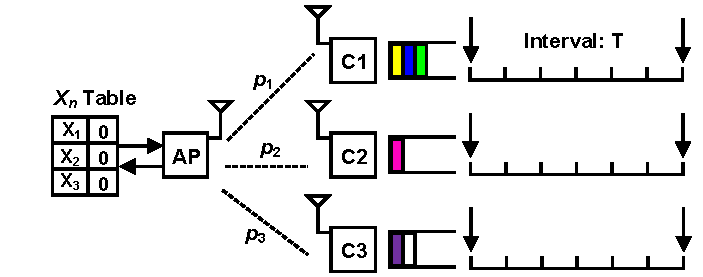
\includegraphics[scale=0.8]{network.pdf}
\end{figure}
\end{frame}

\begin{frame}
\frametitle{Baseline Policy - A Toy Example}
\begin{itemize}
\item $N=3$ and $T=6$
\item $p_1 = p_2 = p_3 = 0.5$
\item Real-time traffic
\item $X_n(k) =$ queue length at the start of the $k$-th interval 
\end{itemize}
\begin{figure}
\centering
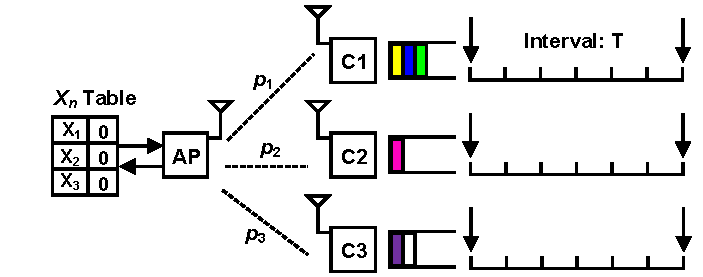
\includegraphics[scale=0.8]{network.pdf}
\end{figure}
\end{frame}

\begin{frame}
\frametitle{Baseline Policy - A Toy Example}
\begin{itemize}
\item Phase 1: AP polls $X_n$ in a round-robin manner
\end{itemize}
\begin{figure}
\centering
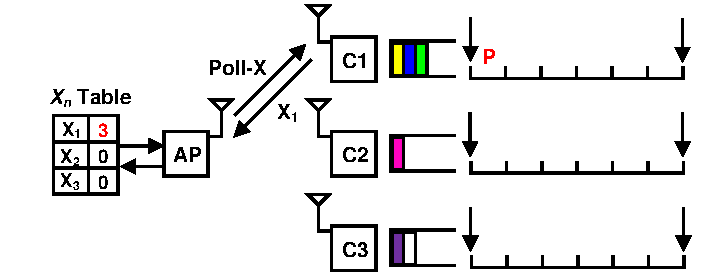
\includegraphics[scale=0.8]{animation_01.pdf}
\end{figure}
\end{frame}

\begin{frame}
\frametitle{Baseline Policy - A Toy Example}
\begin{itemize}
\item Phase 1: AP polls $X_n$ in a round-robin manner
\end{itemize}
\begin{figure}
\centering
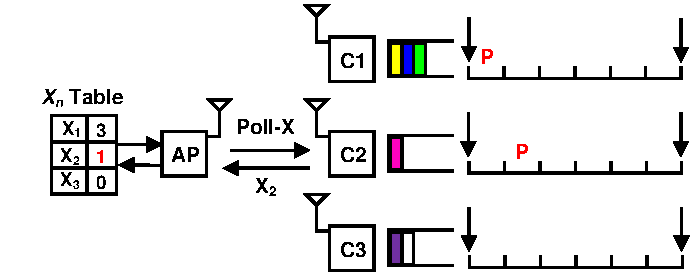
\includegraphics[scale=0.8]{animation_02.pdf}
\end{figure}
\end{frame}

\begin{frame}
\frametitle{Baseline Policy - A Toy Example}
\begin{itemize}
\item Phase 1: AP polls $X_n$ in a round-robin manner
\end{itemize}
\begin{figure}
\centering
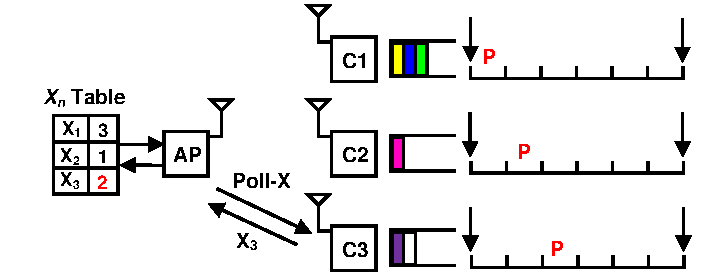
\includegraphics[scale=0.8]{animation_03.pdf}
\end{figure}
\end{frame}

\begin{frame}
\frametitle{Baseline Policy - A Toy Example}
\begin{itemize}
\item Phase 2: AP schedules a client based on Max-Weight policy
\item Max-Weight: select the client that maximizes $p_nX_n$
\end{itemize}
\begin{figure}
\centering
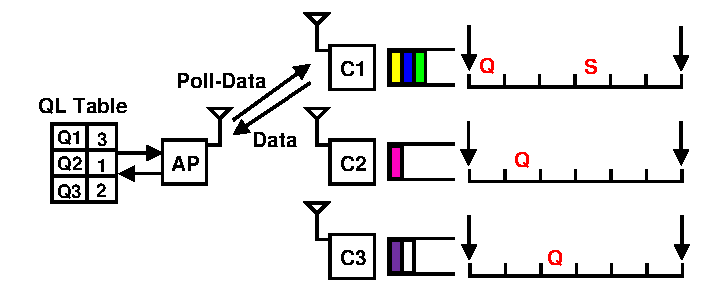
\includegraphics[scale=0.8]{animation_04.pdf}
\end{figure}
\end{frame}

\begin{frame}
\frametitle{Baseline Policy - A Toy Example}
\begin{itemize}
\item Phase 2: AP schedules a client based on Max-Weight policy
\item Max-Weight: select the client that maximizes $p_nX_n$
\end{itemize}
\begin{figure}
\centering
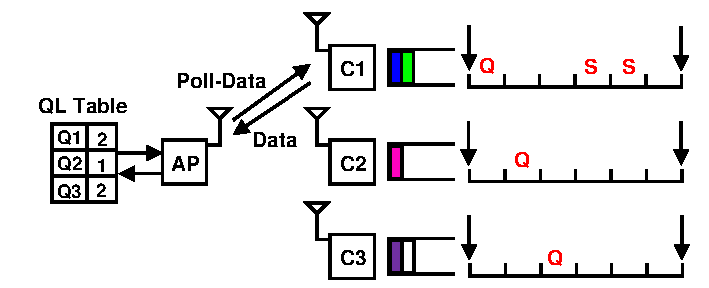
\includegraphics[scale=0.8]{animation_05.pdf}
\end{figure}
\end{frame}

\begin{frame}
\frametitle{Baseline Policy - A Toy Example}
\begin{itemize}
\item Phase 2: AP schedules a client based on Max-Weight policy
\item Max-Weight: select the client that maximizes $p_nX_n$
\end{itemize}
\begin{figure}
\centering
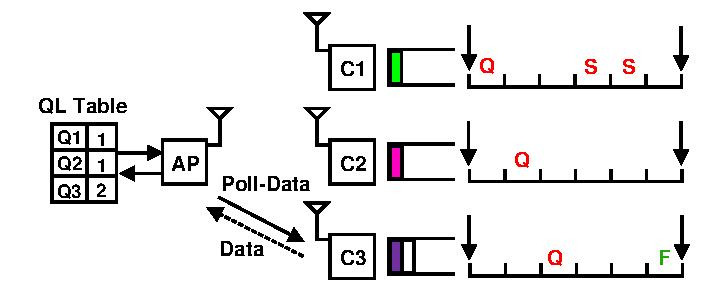
\includegraphics[scale=0.8]{animation_06.pdf}
\end{figure}
\end{frame}

\section{Discussion}

\begin{frame}
\frametitle{Discussion 1}
\begin{itemize}
\item What if Poll-X or $X_1$ is not delivered?
\end{itemize}
\begin{figure}
\centering
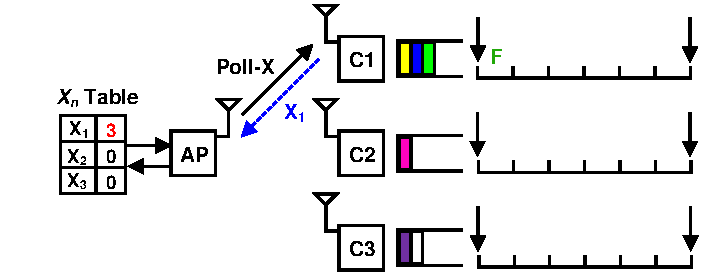
\includegraphics[scale=0.8]{discussion_1.pdf}
\end{figure}
\begin{itemize}
\pause
\item Re-transmit Poll-X until the AP receives $X_n$
\item Option: just set $X_n=0$
\end{itemize}
\end{frame}


\begin{frame}
\frametitle{Discussion 2}
\begin{itemize}
\item How does a client know the DATA packet is delivered?
\item Do we need an application-layer "ACK" for AP? 
\end{itemize}
\begin{figure}
\centering
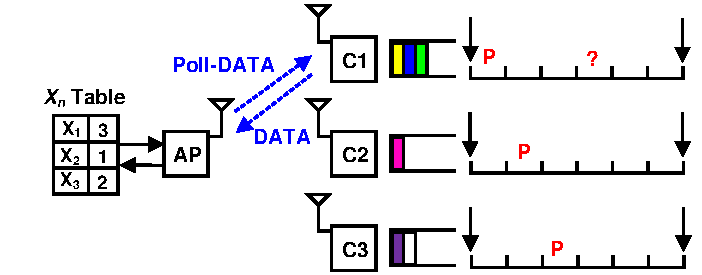
\includegraphics[scale=0.8]{discussion_2.pdf}
\end{figure}
\begin{itemize}
\pause
\item Put "expected packet ID" in Poll-DATA packets
\end{itemize}
\end{frame}

\begin{frame}
\frametitle{Discussion 3}
\begin{itemize}
\item For non-real-time traffic, what does "$X_n$" mean? 
\item There is no application-layer ACK from AP
\end{itemize}
\begin{figure}
\centering
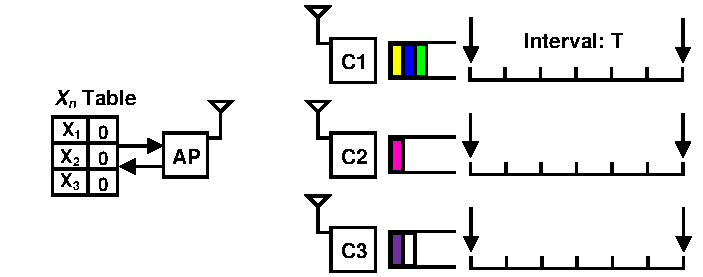
\includegraphics[scale=0.65]{discussion_3.pdf}
\end{figure}
\pause
\begin{itemize}
\item $X_n:=$ total number of packets generated by client $n$
\item $Y_n:=$ total delivery of data packets from client $n$ (maintained by AP)
\item Max-Weight: choose $n$ that maximizes $p_n(X_n-Y_n)$
\end{itemize}
\end{frame}

\begin{frame}
\frametitle{NS-2 Implementation: Packet Types}
\begin{itemize}
\item AP: {\color{red}{Poll-X}} and {\color{red}{Poll-DATA}}
\item Client: {\color{red}{X-Uplink}} and {\color{red}{DATA-Uplink}}
\end{itemize}
\begin{figure}
\centering
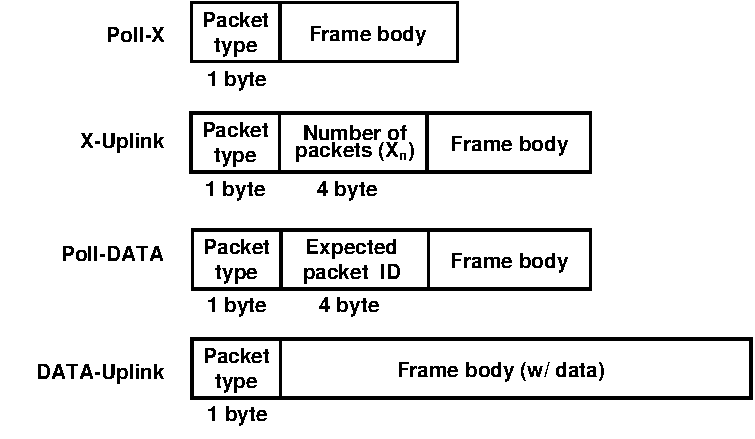
\includegraphics[scale=0.7]{header.pdf}
\end{figure}
\end{frame}

\begin{frame}
\frametitle{NS-2 Implementation: State Machine}
\begin{itemize}
\item AP is controlled by the state machine as follows.
\end{itemize}
\begin{figure}
\centering
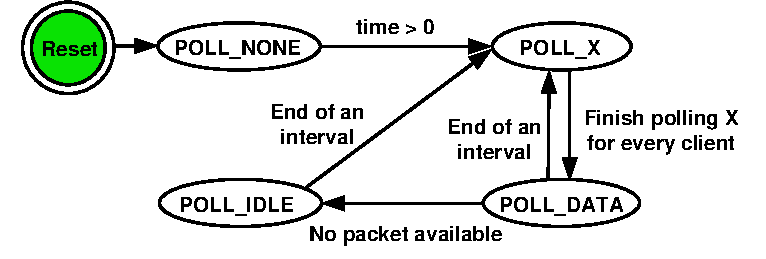
\includegraphics[scale=0.8]{state_machine.pdf}
\end{figure}
\end{frame}


\begin{frame}
\frametitle{Pros and Cons}
\color{blue}{Pros:}
\begin{itemize}
\item Simple polling scheme
\item AP is work-conserving in phase 2 
\end{itemize}
\color{blue}{Cons:}
\begin{itemize}
\item Overhead due to polling
\item Channel utilization for data packets is low
\item Not practical when $N$ is large
\end{itemize}
\end{frame}


\section{Simulation}

\begin{frame}
\frametitle{Simulation Results: Network Capacity}
\begin{itemize}
\item $N=2$ and $T=10$
\item Reliable channel: $p_1 = p_2 = 1$ (symmetric)
\item $N_\text{max}$ ranges from $1$ to $12$
\item Non-real-time traffic
\end{itemize}
\begin{figure}
\centering
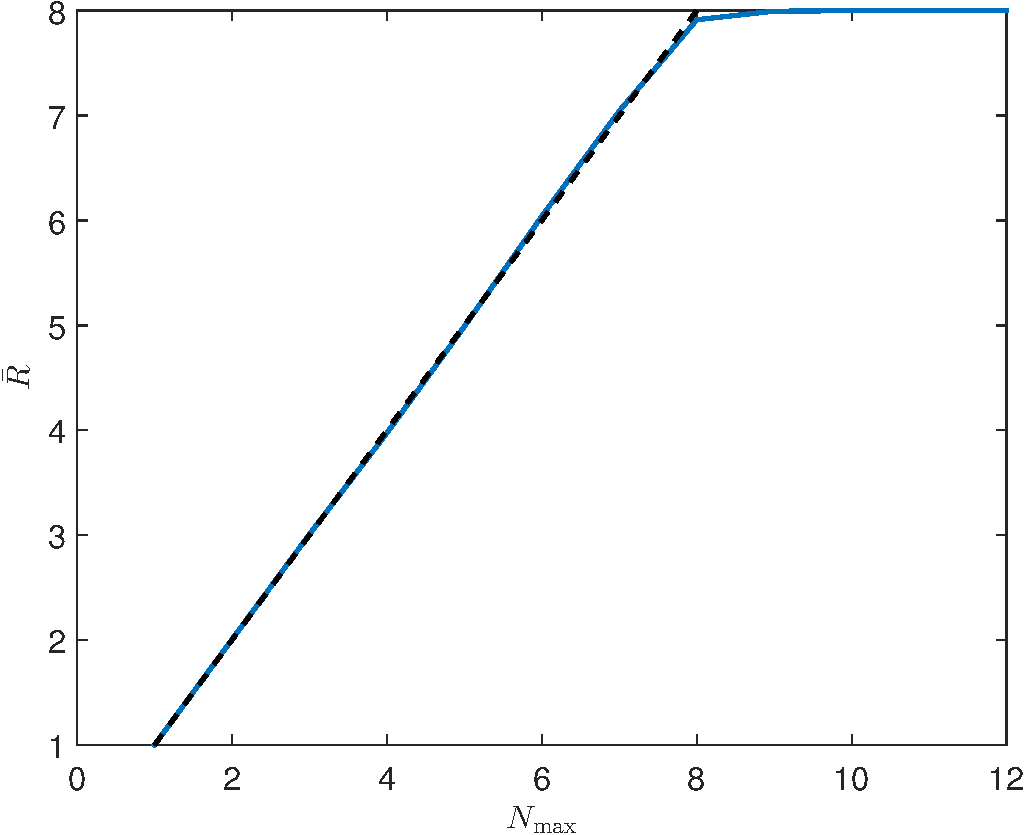
\includegraphics[height=.5\textheight]{nonrealtime_throughput_randmax.pdf}
\caption{Phase 1 polling reduces the capacity.}
\end{figure}
\end{frame}

\begin{frame}
\frametitle{Simulation Results: Network Capacity}
\begin{itemize}
\item $N=2$ and $T=10$
\item Reliable channel: $p_1 = p_2 = 1$ (symmetric)
\item $N_\text{max}$ ranges from $1$ to $20$
\item Real-time traffic
\end{itemize}
\begin{figure}
\centering
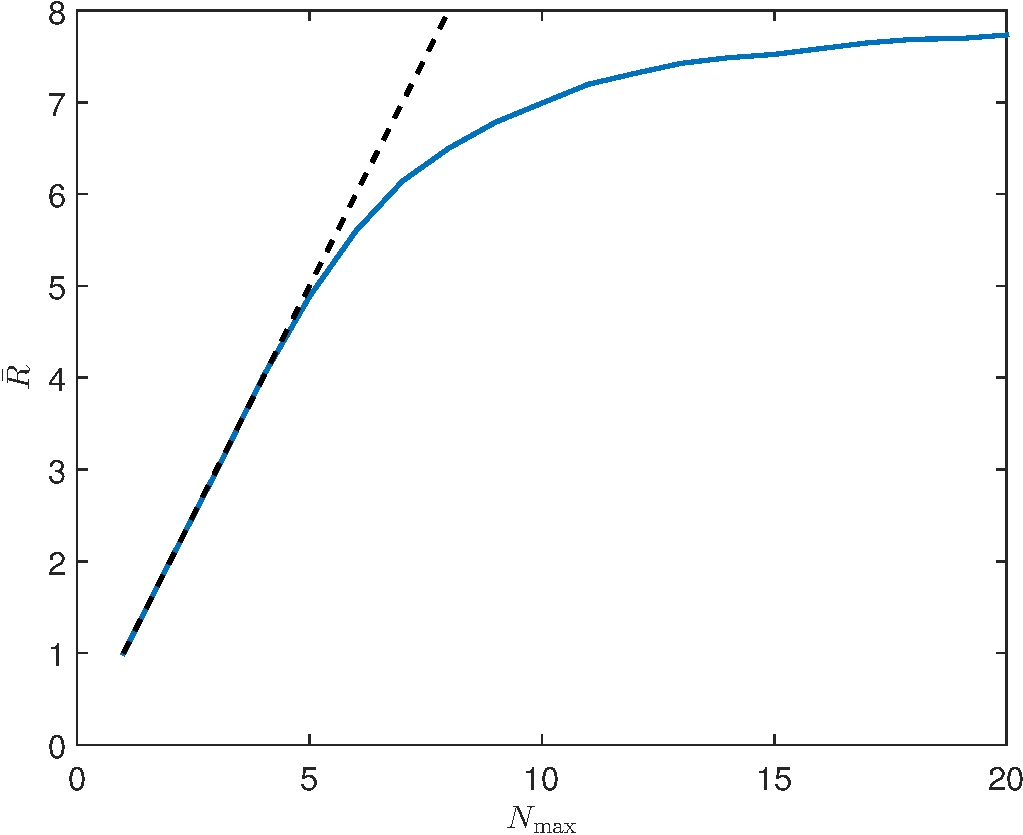
\includegraphics[height=.5\textheight]{realtime_throughput_randmax.pdf}
\caption{Packet deadline reduces the capacity further.}
\end{figure}
\end{frame}

\begin{frame}
\frametitle{Simulation Results: Interval Length}
\begin{itemize}
\item $N=2$
\item Unreliable channel: $p_1 = p_2 \approx 0.57$ (distance \SI{1000}{m})
\item $T$ ranges from $4$ to $16$
\item Non-real-time traffic
\end{itemize}
\begin{figure}[htbp]
  \centering
  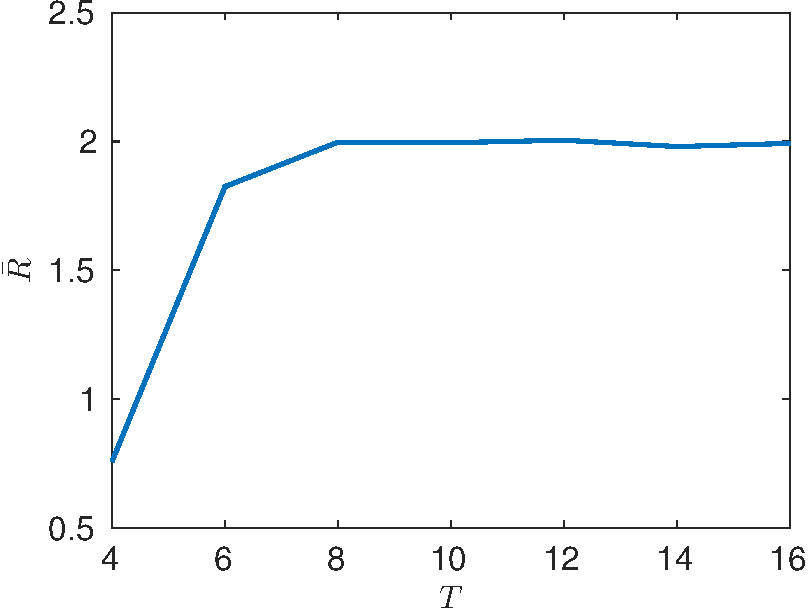
\includegraphics[height=.5\textheight]{nonrealtime_throughput_T.pdf}
  \caption{Interval should be long enough to guarantee deliveries.}
\end{figure}
\end{frame}

\begin{frame}
\frametitle{Simulation Results: Interval Length}
\begin{itemize}
\item $N=2$
\item Unreliable channel: $p_1 = p_2 \approx 0.57$ (distance \SI{1000}{m})
\item $T$ ranges from $4$ to $16$
\item Real-time traffic
\end{itemize}
\begin{figure}[htbp]
  \centering
  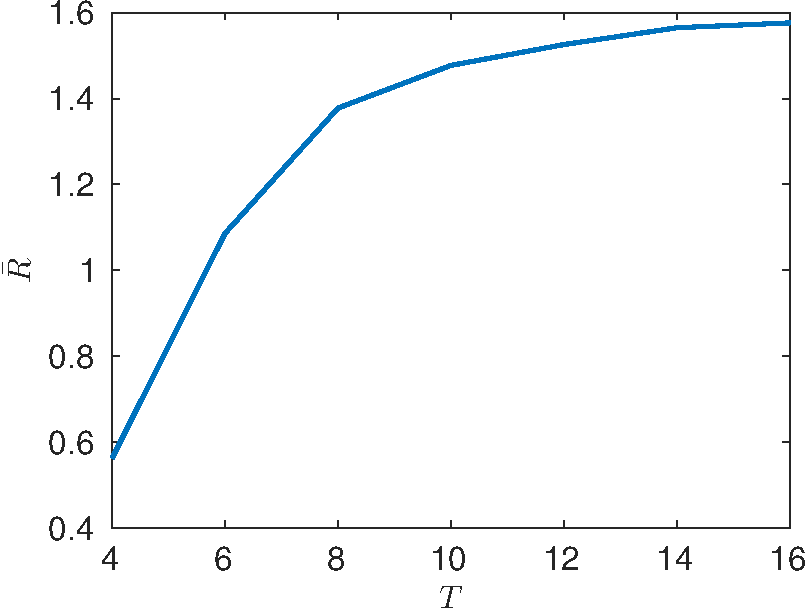
\includegraphics[height=.5\textheight]{realtime_throughput_T.pdf}
  \caption{Interval should be longer when packet can expire.}
\end{figure}
\end{frame}

\begin{frame}
\frametitle{Simulation Results}
\begin{itemize}
  \item Fix $T=10$
\item Unreliable channel: $p_1 = p_2 \approx 0.57$ (distance \SI{1000}{m})
\item $N$ ranges from $1$ to $5$
\item Non-real-time traffic
\end{itemize}
\begin{figure}[htbp]
  \centering
  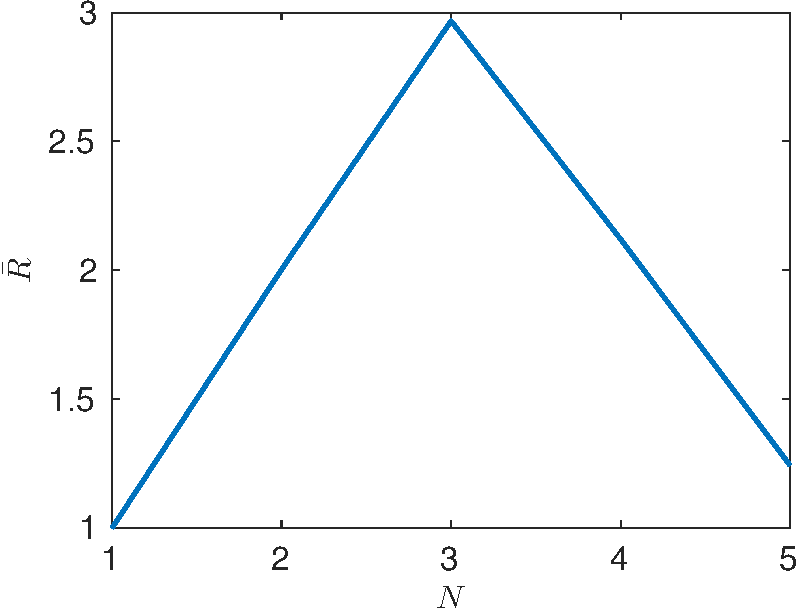
\includegraphics[height=.5\textheight]{nonrealtime_throughput_N.pdf}
  \caption{Performance degrades severely with more clients.}
\end{figure}
\end{frame}

\begin{frame}
\frametitle{Simulation Results}
\begin{itemize}
  \item Fix $T=10$
\item Unreliable channel: $p_1 = p_2 \approx 0.57$ (distance \SI{1000}{m})
\item $N$ ranges from $1$ to $5$
\item Real-time traffic
\end{itemize}
\begin{figure}[htbp]
  \centering
  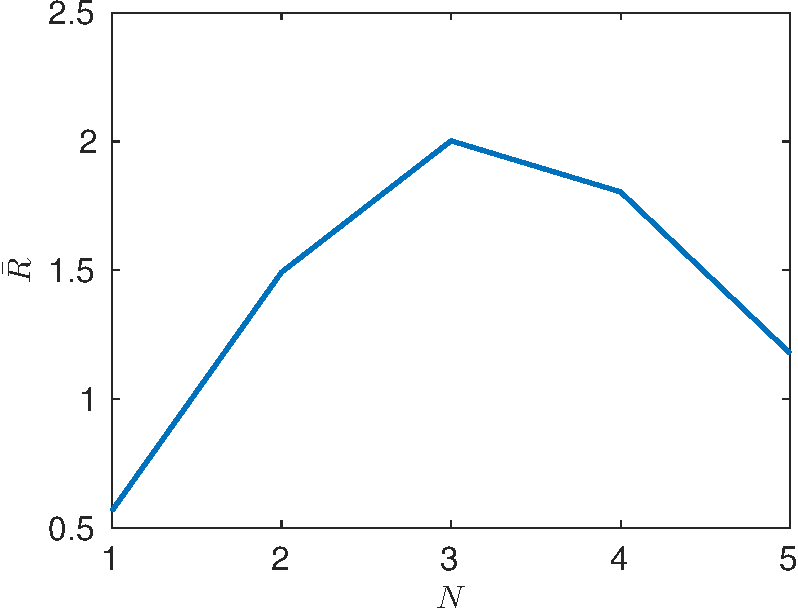
\includegraphics[height=.5\textheight]{realtime_throughput_N.pdf}
  \caption{Performance is worse and also degrades with more clients.}
\end{figure}
\end{frame}

\section*{Conclusion}
\begin{frame}{Conclusion}
  \begin{itemize}
    \item The baseline policy incurs huge overhead especially with large $N$ and small $T$
    \item We need a smarter policy!
  \end{itemize}
\end{frame}


\end{document}
